\section*{Quality Control of raw reads}

Sequencing using \ac{HiFi} resulted in 23.65 Gb of reads, which implies coverage of 31.34x over the \textit{T. vulgaris} genome that has a size of 754.60 Mb according to cytometric estimates.~\cite{marieCytometricExercisePlant1993,PlantDNACvalues} \\

We used LongQC and FASTQC to calculate basic technical statistics and evaluate the quality of \ac{HiFi} raw reads.~\cite{fukasawaLongQCQualityControl2020,BabrahamBioinformaticsFastQC} The length of the 1,747,253 raw reads follows a unimodal distribution with a median size of 13.85kb ($\min = 0.10$kb, $\max = 46.7$kb) \\


The quality reports indicate that there are no significant issues. The only notable observation is the GC distribution, which displayed a bimodal pattern characterized by two peaks at approximately 45\% and 37\%, respectively.\\

We trimmed 25 sequences at 3' and 5' using LongQC. Despite the minimal impact of these, we used the trimmed sequences for the remainder of the analysis. \\

\section*{Exploratory analysis of long reads and reference genome}

When aligning the best five percent of \textit{T. vulgaris }\ac{HiFi} reads to the \textit{T. quinquecostatus} reference genome, we mapped 97.6\% of the reads. The alignment blocks have a median length of 3.2kb ($\min = 0.2$kb, $\max = 61.8$kb).\\

%The median theoretical coverage of chromosomes is 18.1x ($\min = 16.3$x, $\max = 20.5$x). \\

As explained in the corresponding section on methods, we fitted a Zero-Inflated Poisson to the counts' distribution per 1000-length windows using Bayesian inference. The posterior sampling distribution of the parameters is shown in \autoref{fig:bayesian_posterior}. The 95\% credibility interval, computed for all chromosomes, is 0.74-0.77 for $p$, the probability of not coming from the Poisson process, and 2.02-2.51 for $\lambda$, the rate of mapped reads per window. \\

\graphicspath{{gfx/}}
\begin{sidewaysfigure}
\begin{center}
    \input{gfx/05-posterior_var_edited.pdf_tex}
    \caption{Posterior sampling distribution of the parameters of a zero-inflated Poisson model}    
    \label{fig:bayesian_posterior}    
\end{center}
\footnotesize
The posterior sampling distributions of $p$ and $\lambda$ were obtained by modeling the number of mapped reads per 1000-length windows according to the model specified by Equation \eqref{eq:model} using an \ac{MCMC}.   
\end{sidewaysfigure}    

Although not included in this report, we experimented with different subset sizes, alignment tools, and window sizes. These experiments produced consistent results. We have decided to use Minimap2 with default parameters, as it is the standard in the field.\\

Regarding the number of iterations and chains, various experiments with both experimental and simulated data justified a conservative choice, as we obtained equivalent results in all cases using fewer computational resources. \\

\section*{De novo assembly}

As discussed in Methods, a \textit{de novo} assembly from our \ac{HiFi} reads was available before starting the project. \\

As mentioned earlier, \textit{T. vulgaris} haploid genome size is 754.60 Mb.~\cite{marieCytometricExercisePlant1993,PlantDNACvalues} The total size of our \textit{de novo} assembly exceeds the estimate by 20\%; 911.87Mb.

\section*{Homology-based assembly scaffolding}

We generated scaffolds using RagTag, according to a whole-genome alignment of the \textit{de novo} contigs against \textit{T. quinquecostatus} assembly. \autoref{fig:coverage_long_reads} displays the whole genome alignment coverage of \textit{T. quinquecostatus}. \\

The alignments cover most of the start and end of the 13 pseudo-chromosomes but present large uncovered areas, especially near the middle of the pseudo-chromosome. In total, 47.3\% of the \textit{T. quinquecostatus} genome is uncovered. This fact is consistent with the Zero-inflated poisson model discussed above.\\

\begin{figure}[h]
    \begin{center}
        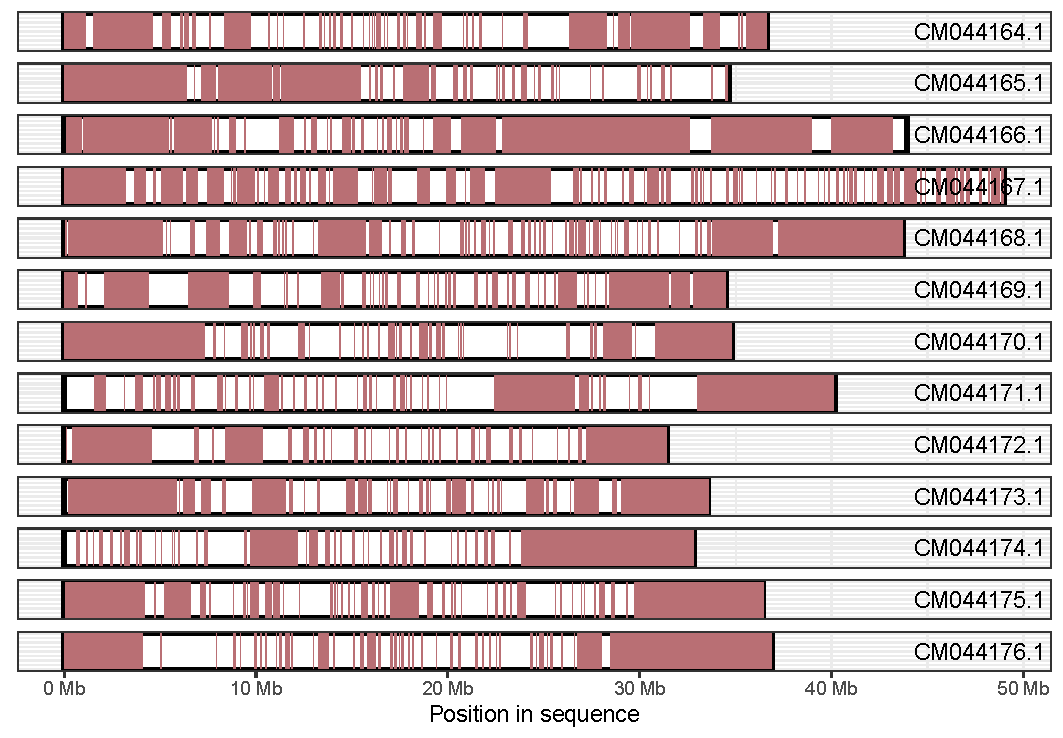
\includegraphics[width=\textwidth]{gfx/coverage_long_reads_tq.pdf}
        \caption{Covered areas of \textit{T. quinquecostatus} by the whole-genome alignment between \textit{T. vulgaris} and \textit{T. quinquecostatus}}   
        \label{fig:coverage_long_reads}
 
    \end{center}
        \footnotesize
    Covered areas are shown in red. We include only primary alignments whose length is larger than 1000, as those are the ones RagTag will use for the scaffolding process. We represent the alignments only to the 13 pseudo-chromosomes.  
\end{figure}   

We used the whole-genome alignment to orient and arrange the different contigs into larger scaffolds (see \autoref{fig:sinteny} for an example). The scaffolding process placed 77\% of base pairs into scaffolds. Interestingly, a few contigs aligned not to the \textit{T. quinquecostatus} pseudo-chromosomes but to its unplaced contigs.\\
 

\begin{figure}
\begin{center}
    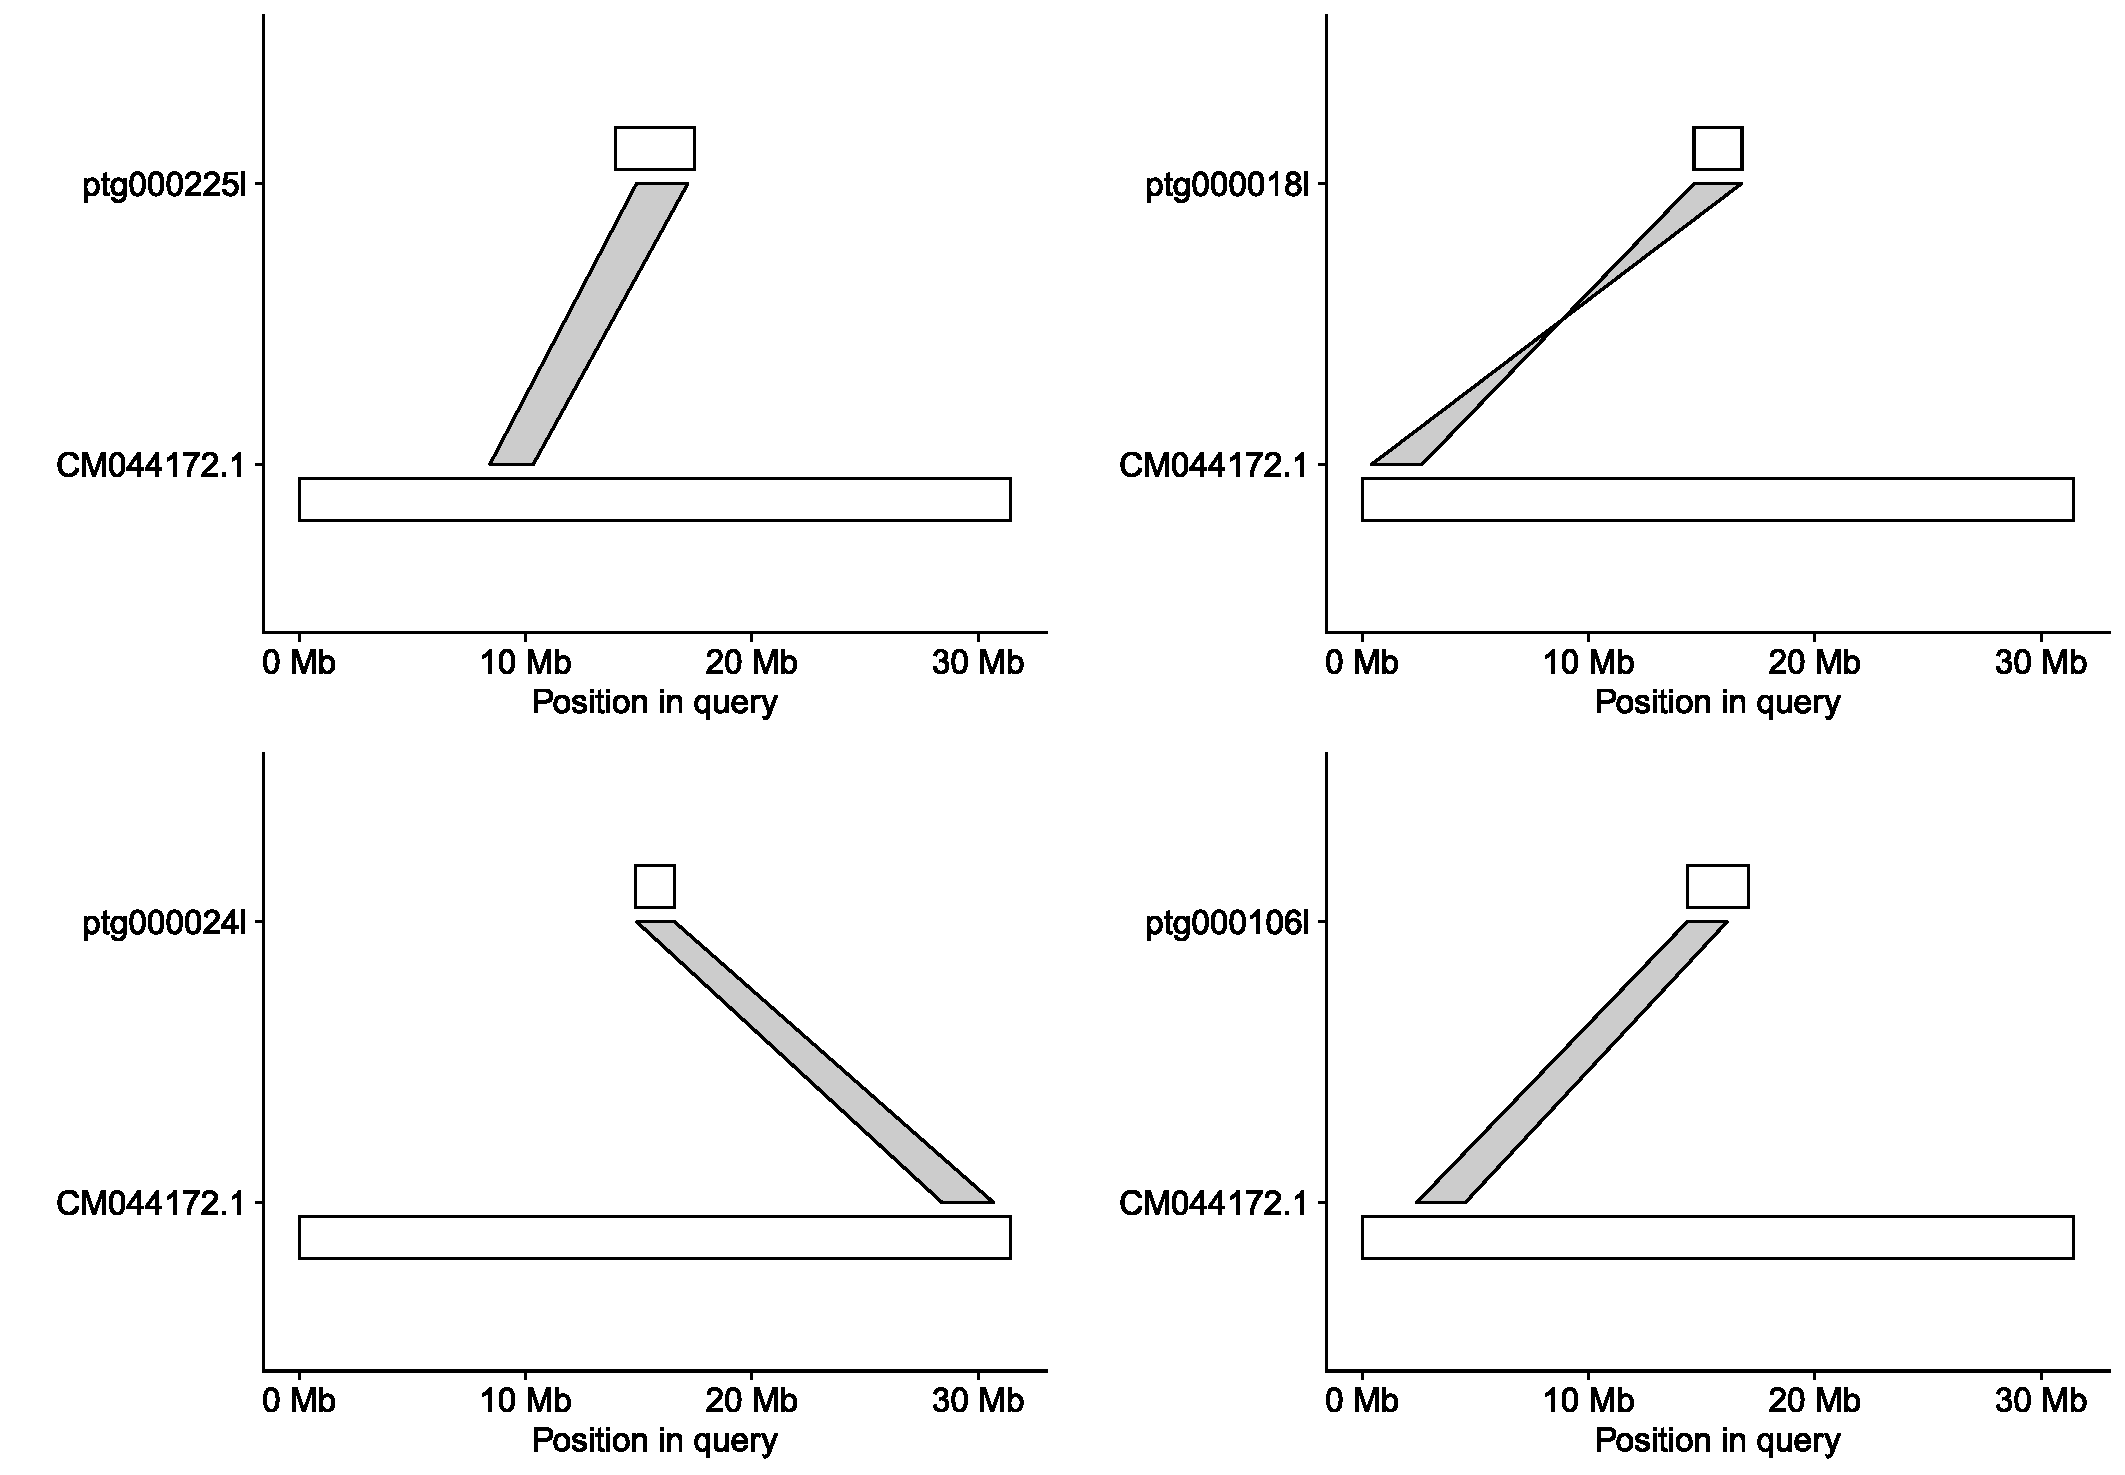
\includegraphics[width=\textwidth]{gfx/CM044172.1_sinteny.pdf}
    \caption{Sinteny-like plot of pseudo-chromosome CM044172.1}  
    \label{fig:sinteny}    
\end{center}
\footnotesize
We show the alignments of the largest four \textit{de novo} contigs of \textit{T. vulgaris} mapped to  CM044172.1 pseudo-chromosome of \textit{T. quinquecostatus}. This visualization corresponds to arranging and orienting the contigs in the scaffolding process. 
\end{figure} 

The scaffolded assembly has 819 gap sequences. When possible, we calculated the gap sizes according to Equation \eqref{eq:infergapsize} and the whole-genome alignment. In most cases, we could not estimate the gap size because the inferred size was greater than the threshold established.\\

We are certain of the size of 8.3\% of the gaps; the rest have arbitrary lengths. As expected, given the spatial distribution of the coverage (see \autoref{fig:coverage_long_reads}), most gaps with unknown sizes are found in the middle of the scaffolds.\\

In summary, we reconstructed 13 superscaffolds (pseudo-chromosomes) by merging adjacent contigs from the assembly that aligned to each of the 13 pseudo-chromosomes of \textit{T. quinquecostatus}, supported by \ac{Hi-C} experimental data. This reconstruction was guided by the homology observed between \textit{T. quinquecostatus} and \textit{T. vulgaris}.\\

\section*{Assembly quality assessment}

We show global statistics comparing the assembly at a contig and scaffold level in \autoref{tab:global}. The scaffolding has proven highly effective, as the final assembly has a contig N50 of 1.87 Mb and a scaffold N50 of 48.92 Mb. \\

%This fact supports the reliability of the pseudochromosomes obtained. \\

\begin{table}[h!]
    \begin{minipage}{\linewidth}
    \renewcommand\thefootnote{\thempfootnote}
    \centering
    \begin{tabular}{@{}cccccc@{}}
        \toprule
        & N\#    & Ave (Mb) & Largest (Mb)& N50 (Mb)\footnote{Length such that scaffolds/contigs of this length or longer include half the bases of the assembly.}     & Ns\footnote{Number of Ns (ambiguous nucleotides)}      \\ \midrule
        Contigs      & 1,884 & 0.48     & 11.17        & 1.87 ($n$=133) & 0       \\
        Scaffolds & 1,065 & 0.86     & 95.24        & 48.92 ($n$=8)  & 2,536,928 \\ \bottomrule
        \end{tabular}
        \caption{Global statistics of the assembly at contig and scaffold level}
        \label{tab:global}
\end{minipage}
\end{table}

BUSCO analysis assesses the genome assembly completeness by examining the expected gene content of universal orthologs. The analysis produced the following results: C:96.4\%[S:65.0\%,D:31.4\%], F:0.6\%, M:3.0\%, n:2326.\\

The completeness score, 96.4\%, is only slightly lower than the one obtained by Sun \etal~\cite{sunChromosomelevelAssemblyAnalysis2022} for \textit{T. quinquecostatus}, which is the closest assembly available. However, the percentage of complete and duplicated genes in \textit{T. vulgaris} is significantly higher at 31.4\% compared to \textit{T. quinquecostatus}, which is only 4.5\%. Using it for scaffolding does not affect this result, as we are not modifying the original sequence.\\

Lastly, the total size of our 13 pseudo-chromosomes is 695.63 Mb, considerably closer to the cytometric estimation of  754.60 Mb than the overall size of the \textit{de novo} assembly.  \\


\section*{Mapping short Illumina reads to scaffolds}


We used available Illumina sequences of the five individuals (from \textit{T. vulgaris} and \textit{S. montana}) to validate our assembly with independent experimental data. \autoref{fig:error_rate} shows the result of this experiment.\\

Reads have been sequenced using a targeted enrichment protocol. Thus, we can not use the coverage to validate our reference genome, given that it will be arbitrarily low if the enrichment process works adequately. Instead, we will look at differences in the percentage of properly aligned sequences and the number of mismatches compared to the reference.\\

\begin{figure}
    \begin{center}
        \def\svgwidth{\textwidth}
        \input{gfx/mapped_vs_error_rate.pdf_tex}
        \caption{Aligned short Illumina reads to the \textit{T. vulgaris} assembly}            
        \label{fig:error_rate}
    \end{center}
    \footnotesize
    We show the fraction of mismatches against the percent of properly paired reads for five individuals and two hybridization protocols. We considered a read properly paired if both forward and reverse reads are consistent in orientation and distance according to samtools criterion.~\cite{danecekTwelveYearsSAMtools2021} An ellipse indicates the reads of THc607, which was also sequenced using \ac{HiFi} to construct the assembly.
\end{figure}  

The two \textit{S. montana} individuals are grouped in \autoref{fig:error_rate}, showing similar mapping patterns to the scaffolded assembly of \textit{T. vulgaris}. They have a lower percentage of properly mapped sequences than the other \textit{T. vulgaris} specimens. Hybridization two, the more stringent procedure, increases the percentage of mapped reads and the number of mismatches in both \textit{S. montana} individuals.\\

The increased number of mapped reads also affects \textit{T. vulgaris} individuals, but it is less pronounced. Hybridization two does not increase the number of mismatches in \textit{T. vulgaris} as it does in \textit{S. montana}. The differences in the percentage of mapped reads between \textit{T. vulgaris} individuals are slight, but the individual Thym607 used to construct the assembly has the lowest number of mismatches.